\chapter{Smart Contract Security}

\section{Introduzione}

Come per altri programmi, un Smart Contract eseguirà esattamente ciò che è scritto,
che non sempre è ciò che il programmatore intendeva. Tutti i contratti smart sono
pubblici e qualsiasi utente può interagire con essi semplicemente creando una
transazione.
Una volta che la transazione viene mandata sulla blockchain, significa che fa parte
di un blocco e non può essere più annullata.
I dati della transazione sono inalterabili anche perchè
sono distribuiti.
Gli Smart Contract possono gestire denaro, ma una volta perso è praticamente
impossibile recuperarlo.
Il codice dello Smart Contract è spietato. Ogni bug può portare a perdite
monetarie.
La complessità è nemica della sicurezza. Più semplice è il codice,
minori sono le possibilità
che si verifichi un bug o un effetto imprevisto. Quando ci si impegna per la
prima volta nella
programmazione di uno Smart Contract, gli sviluppatori sono spesso tentati di
provare a scrivere codice molto codice ed articolato.
Invece, si dovrebbe trovare il modo per fare meno, con meno linee di
codice, meno complessità e meno "features".
Se esiste già una libreria o un contratto che fa gran parte del necessario,
riutilizzatela.
All'interno del codice, seguite il principio \textit{DRY}: Don't Repeat Yourself.
Attenzione alla sindrome del "Not Invented Here", dove si è tentati di
"migliorare" una caratteristica o un componente costruendola da zero.
Non si dovrebbe trattare la programmazione a Smart Contract allo stesso modo della
programmazione generale. Piuttosto, si dovrebbero applicare rigorose metodologie di
ingegneria e di sviluppo software.
Una volta "lanciato" il vostro codice, c'è poco da fare per risolvere eventuali
problemi.
Il vostro codice deve essere chiaro e facile da comprendere.
Più è facile da leggere, più è
facile da controllare.
I contratti intelligenti sono pubblici, poiché tutti possono leggere il bytecode
e chiunque può
invertirlo e modificarlo. Pertanto, è utile sviluppare il proprio lavoro in
pubblico, utilizzando
metodologie collaborative e open source, per attingere alla saggezza collettiva.
Dato che l'ambiente di esecuzione è pubblico, prima di poter essere lanciato,
il codice deve essere
testato in maniera approfondita.
Vanno soprattutto analizzati i possibili input maligni e i loro effetti.

\section{IF e REQUIRE}

\begin{lstlisting}
    if(_newDelegate != delegateContract){
        // Do something
    }

    require(_newDelegate != delegateContract){
        // Do something
    }
\end{lstlisting}

\paragraph{IF.}
È solo un'esecuzione condizionale del blocco \verb|// Do something|.
Quindi, se questa condizione non
è soddisfatta, \verb|// Do something| viene saltato.

\paragraph{REQURIE.}
Controlla sempre una condizione ma,
se non si avvera, la transazione viene abortita e
ripristinata. Viene rimborsato anche il gas.
\ \\
\paragraph{Esempio.}\

\begin{lstlisting}
uint256 input;
address sender;
function some_state_changing_fn(uint256 _input) public 
  returns (bool success) {
     sender = msg.sender;
     require(_input >= 100);
     input = _input;
     success = true;
}
\end{lstlisting}

\verb|sender| è l'indirizzo di chi chiama la transazione e spedisce denaro.
Il corpo della funzione salva in \verb|sender| l'indirizzo \verb|msg.sender|.
\verb|msg| è il messaggio che viene
mandato al contratto. \verb|require| richiede che l'input passato sia $ > 100$.
Se il valore passato \verb|_input| nella transazione è $ > 100$,
allora si aggiorna la variabile \verb|input|.
Altrimenti fallisce. Aggiornando \verb|input| si aggiorna lo stato del contratto.

\section{DAO Attack}

\subsection{Reentrancy}

Una delle caratteristiche degli Smart Contract di Ethereum è la loro capacità di
richiamare e utilizzare il codice di altri contratti esterni. I contratti
gestiscono l'ether e spesso lo inviano a
vari indirizzi di utenti esterni. Queste operazioni richiedono ai contratti di
inviare appunto call esterne.
Queste chiamate possono essere dirottate dagli aggressori, i quali potrebbero
costringere i contratti ad eseguire ulteriori codici
(attraverso una funzione di fallback). Attacchi di questo
tipo sono stati utilizzati nel famigerato hack DAO.
Il 17 giugno 2016 il DAO è stato violato e $3,6$ milioni di ether ($658.002.709$ euro)
sono stati rubati con quello che viene considerato i primo attacco di reentrancy.

\subsection{Attacco}

In Solidity esistono 3 funzioni per il trasferimento di ether: \verb|someAddress.send()|,
\verb|someAddress.transfer()| e \verb|someAddress.call.value()|.
Da notare che \verb|x.transfer(y)| è equivalente a \verb|require(x.send(y))|.
\verb|send| e \verb|transfer| sono sicure contro il \textit{reentrancy} perché
hanno associato un certo limite di operazioni possibili.
Infatti, se la funzione eseguita consuma più del limite imposto da \verb|send| e \verb|transfer|,
si interrompe l'esecuzione.
Al contratto chiamato viene assegnato solo uno valore di $2300$
gas, sufficiente solo per registrare un certo evento.
Il gas in generale permette di evitare DoS. Dovendo gestire pagamenti,
si fa in modo che le chiamate a funzioni dei contratti siano limitate, è un modo
per proteggere la blockchain.
Se la transazione fallisce, viene effettuata un'operazione di ripristino (revert)
automatico, cioè si ritorna allo stato originale.\\
A differenza delle due precedenti, \verb|someAddress.call.value(y)()| non ha questo
tipo di protezione, invocandola verrà inviato
l'ether specificato e farà scattare
l'esecuzione di una specifica perte di codice del contratto chiamante
(funzione di \textit{fallback}).
Il codice eseguito viene fornito con tutto il gas
disponibile per l'esecuzione, rendendo
questo tipo di trasferimento di valori unsafe contro il reentrancy.
Non ci sono quindi limiti, si può andare anche oltre $2300$ gas.

\paragraph{ESEMPIO.}\ \\
\verb|contract.sol|\\
Di seguito il codice di uno Smart Contract simile a quello del DAO Attack.

\begin{figure}[H]
    \centering
    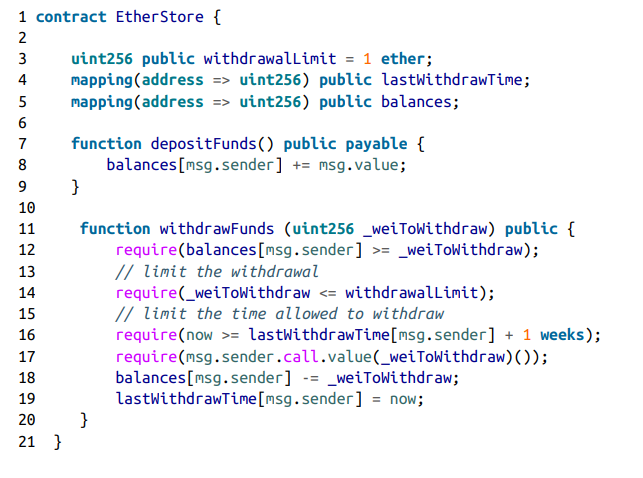
\includegraphics[width=10cm, keepaspectratio]{capitoli/ethereum/imgs/dao_buono.png}
    \caption{Codice del contratto contract.sol}
\end{figure}

Abbiamo due funzioni. La prima, \verb|depositFunds|, permette di depositare
appunto i fondi.
La funzione ha l'attributo \verb|payable|: fornisce un meccanismo per
raccogliere/ricevere fondi in ether per il contratto.
Nella funzione viene aggiornato il bilancio del mittente con \verb|msg.value|.
\verb|balance| è un array dei depositari, mentre \verb|msg.value| indica la
quantità di ether che viene trasferita.
La funzione \verb|withdrawFunds|, invece, serve per ritirare.
Prende come parametro una certa quantità di denaro.
Ha una serie di \verb|require|:

\begin{enumerate}
    \item Richiede che il bilancio depositato sia maggiore di quello ritirato;
    \item Il bilancio ritirato deve essere minore di un certo limite
          (stabilito arbitrariamente);
    \item Verifica che sia passato del tempo dall'ultima richiesta di ritiro di
          denaro;
    \item Trasferisce gli wei attraverso la funzione \verb|msg.sender.call.value|
          che non ha limiti sul gas;
\end{enumerate}

Alla fine si aggiorna il bilancio di \verb|msg.sender| e lo stato interno,
compreso il momento in
cui è avvenuta la transazione (\verb|now|).\ \\

\verb|attack.sol|\ \\
Di seguito il codice del contratto scritto per attaccare il precedente.

\begin{figure}[H]
    \centering
    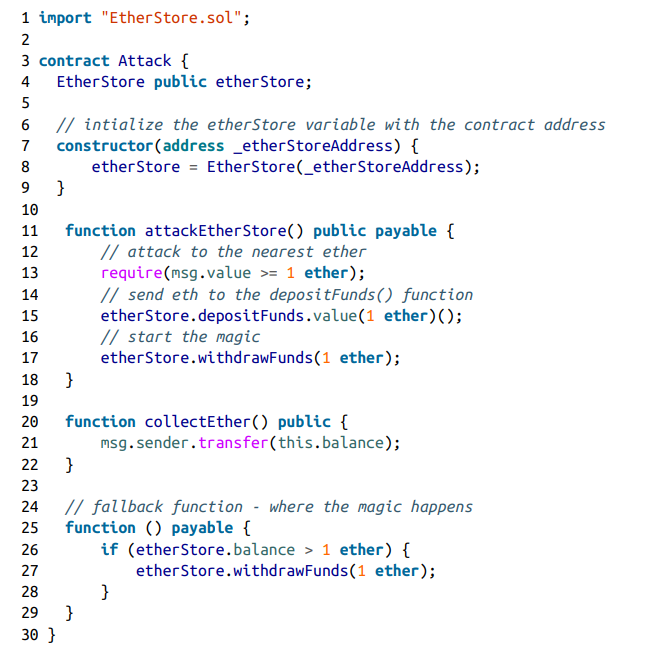
\includegraphics[width=10cm, keepaspectratio]{capitoli/ethereum/imgs/dao_cattivo.png}
    \caption{Codice del contratto attack.sol}
\end{figure}

Il costruttore viene inizializzato con l'indirizzo del contratto che si vuole
attaccare: viene memorizzato nella variabile \verb|etherStore| e quindi
chiaramente anche nella blockchain.
Il trasferimento di denaro avviene tramite la funzione \verb|collectEther|.
Chiamo il contratto e
quindi anche questa. Trasferisco una certa quantità di ether $ >=1$
(per come stabilisce il \verb|require|). L'Ether viene inviato a \verb|etherStore|,
cioè il contratto che si vuole attaccare.
Sul contratto di attacco c'è depositato 1 ether.
Gli chiedo di aggiungerne 1 altro sul precedente chiamando \verb|withdrawFunds|.
Avviene quindi il versamento e poi l'ulteriore
richiesta.
Se non viene specificata una funzione in particolare,
viene chiamata di default la fallback.
Le funzioni di fallback in Solidity vengono eseguite quando un identificatore di
funzione non corrisponde a nessuna delle funzioni disponibili in un contratto
oppure se non sono stati
forniti dati. Sono senza nome, non possono accettare argomenti, non possono
restituire nulla e ci può essere solo una funzione di fallback.
Sono una sorta di valvola di sicurezza.
In breve, il contratto di attacco ha versato 1 ether ma allo stesso tempo sta
effettuando più volte di seguito la richiesta di ritirarne 1.
Il problema è che l'aggiornamento del \verb|balance| viene
effettuato soltanto dopo la spedizione del denaro. Per cui (per esempio) invece
di chiederne 1 ne chiedo e ne ricevo 2.
Ritiriamo di più di quanto effettivamente richiesto.
La funzione in realtà sta aspettando una risposta e il conseguente aggiornamento, ma
vengono solo sottratti ulteriori ether. L'attacco va a buon fine in quanto il controllo sul
bilancio viene effettuato soltanto alla fine.

\paragraph{RICAPITOLANDO.}\ \\
Per sfruttare la vulnerabilità dovuta dalla funzione \verb|someAddress.call.value()|
procedo nel seguente modo:

\begin{enumerate}
    \item Effettuo una transazione al contratto malvagio (\verb|attack.sol|) di almeno
          1 ether (\verb|require| alla riga 13 di \verb|attack.sol|)
    \item 1 ehter viene depositato sul contratto bersaglio (\verb|contract.sol|) invocando
          la funzione \verb|depositFunds| (riga 15 di \verb|attack.sol|)
    \item Chiedo al contratto bersaglio di ritirare i fondi che ho depositato
          (riga 17 di \verb|attack.sol|). È proprio qui che inizia la \textit{magia}.
    \item  Viene eseguita la funzione \verb|withdrawFunds| (riga 11 di \verb|contract.sol|).
          Tutti i \verb|require| vengono superati e viene inviato il denaro al contratto attaccante
          (riga 17 di \verb|contract.sol|).
    \item Questo invio non fa continuare l'esecuzione della funzione \verb|withdrawFunds|
          andando a modificare il bliancio, ma triggera l'esecuzione della funzione
          di fallback del contratto attaccante.
    \item  Viene eseguita la funzione di fallback del contratto attaccante
          (riga 25 di \verb|attack.sol|) che continuerà a richiedere soldi
          (e li otterrà) fin
          quando il bilancio del contratto bersaglio non finirà, impedendo
          per tutto il tempo che la riga 18 di \verb|contract.sol| venga eseguita.
\end{enumerate}

\subsection{Mitigation}

Per cercare di arginare questa falla si usa una combinazione di più accorgimenti:

\begin{enumerate}
    \item Usiamo una mutex, ovvero una variabile booleana subito all'inizio
          del ritiro. Altrimenti chi ha chiamato continuerebbe a farlo senza problema.
          Se la variabile booleana è
          settata nel modo corretto (all'inizio è a false), si bloccano gli accessi.
          Non si entra nel
          contratto se la mutex non è stata sbloccata.
    \item Aggiorno il bilancio prima di trasferire i soldi al chiamante.
          Prima trasferivo i soldi e
          poi aggiornavo il bilancio, ora il contrario.
          Cio è accompagnato dallo sblocco del
          mutex.
    \item Viene usata la \verb|transfer| con il suo limite di gas che causa
          quindi un limite per l'
          esecuzione.
\end{enumerate}